%%%%%cas simple d'un blindage avec des conducteurs %%%%%%%%%
\begin{frame}
\frametitle{Cas simple d'un blindage avec des conducteurs}
\begin{columns}[T]
\column{0.35\linewidth}
\begin{center}
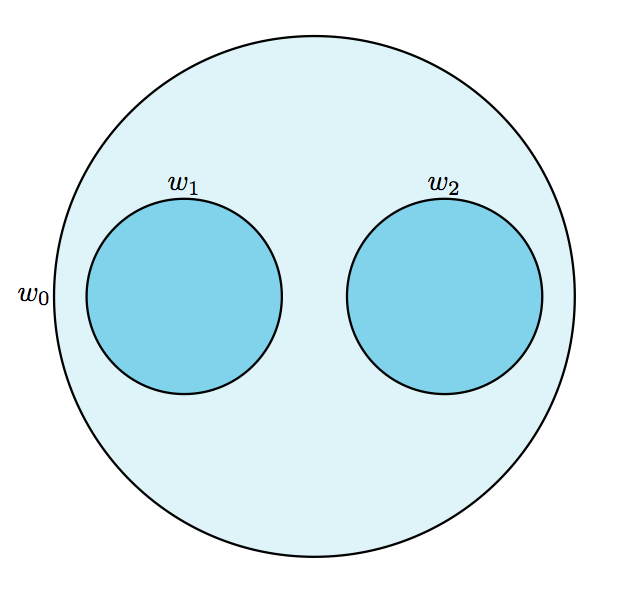
\includegraphics[scale=0.2]{figures/f3}
\end{center}
\column{0.65\linewidth}
Blindage de r\'er\'erence $w_0$, $2$ conducteurs $w_1, w_2$
\begin{itemize}
\item $1^{ere}$ \'etape : calcul $\varphi_i$ avec $i=1,2$-solution de
 \begin{equation}
 \begin{cases}
 -\Delta\varphi_i = 0 \quad \text{sur } \Omega \\
 \varphi_i =  
 \begin{cases}
 1 \quad \text{sur } w_i \\
 0 \quad \text{sur } \{w_0,w_1,w_2 \} \setminus w_i
 \end{cases}
 \end{cases}
 \end{equation}
\item $2^{ere}$ \'etape : Chercher des fonction test $\psi_i$ pour chaque $\varphi_i$
\item $3^{ere}$ \'etape : Caculer les coefficients de la matrice $M$
\begin{equation}
M_{ij} = \int_{w_i} -\Delta\varphi_j \psi 
\end{equation}
\item $L_{ext}$ : matrice d'inductance des conducteurs ext\'erieurs  
\end{itemize}
\end{columns}
\end{frame} 

%%%%%cas simple des blindage avec des conducteurs (2 niveaux) %%%%%%%%%